\chapter{Музыка? Нет, не слышали\ldots}
\label{ch:music}

Сейчас мы зайдем на территорию музыки, вооружившись инструментами математики и физики. Читатель спросит: неужели мы начнем войну разума и чувств, науки и искусства? Нет и нет! Наоборот, мы будем наводить мосты дружбы между ними! 

Музыка отражает красоту математики, существующей \emph{внутри} нас, с помощью физики, существующей \emph{снаружи}. Музыка --- это один из способов передать математическую гармонию \emph{внутреннего} мира человека в несколько хаотичный \emph{окружающий} его мир.

А для тех, кто действительно не слышал музыку, дадим простое определение:

\begin{Definition}[Музыка]
    Музыка\index{музыка} начинается тогда, когда звуки \emph{правильной} высоты с \emph{правильной} громкостью появляются в \emph{правильное} время
\end{Definition}

Давайте разбираться с музыкальными \emph{правилами}!


\section{Что да как? Немного физики}
\label{ch:music:physics}

Если задеть гитарную струну, вы услышите \emph{звук}\index{звук}. Струна колеблется и создает вокруг себя периодические сжатия и разряжения воздуха, которые распространяются во все стороны от струны. Этот эффект называется звуковой \emph{волной}\index{звуковая волна}. По воздуху звуковая волна распространяется от источника со скоростью примерно\footnote{Скорость звука зависит от температуры, давления и влажности воздуха. В общем случае скорость звука зависит от проводящей этот самый звук среды, например, в воде звук распространяется гораздо быстрее, чем в воздухе} 340 метров в секунду.

Количество периодических сжатий (или разряжений) в секунду физики называют \emph{частотой}\footnote{Единица измерения частоты --- Герц. Сокращенно --- Гц. 1Гц --- одно колебание в секунду. 400Гц --- четыреста колебаний в секунду}, а лирики --- \emph{высотой}\index{звук!высота} звука. Чем чаще колеблется струна, тем \emph{выше} звук, который она издаёт. Ну и наоборот: чем реже колеблется струна, тем \emph{ниже} звук. Верхние струны на гитаре (шестая, пятая и четвертая), издающие относительно низкие звуки, называются \emph{басовыми}\index{струна!басовая}.

Если вы дёрнете ту же струну сильнее, то она зазвучит \emph{громче}. При этом она издаст звук той же высоты, что и раньше. Но она будет совершать колебания с б\'{о}льшим размахом --- физики скажут: <<с б\'{о}льшей амплитудой>>. Сжатия и разряжения воздуха усилятся. И, когда звук дойдет до уха слушателя, эти сжатия и разряжения начнут сильнее шатать барабанную перепонку в его ухе и\ldots Тут физика кончится, и начнутся биология и биоинформатика --- в эти дебри не полезем.

Человеческое ухо прекрасно улавливает частоту и амплитуду звуковой волны. Незатухающие колебания одной неизменной частоты, человек услышит как тон\footnote{Например, заходящий на посадку на ваше ухо комар, машет крыльями примерно 659 раз в секунду и вы слышите незабываемое Ми второй октавы!}. А амплитуду волны (размах колебаний) --- как громкость\index{звук!громкость}. 

Слуховой аппарат человека воспринимает ограниченный диапазон частот: примерно от 16 до 20000 Гц, а \emph{восприятие} громкости звука, если честно, зависит не только от амплитуды звуковых колебаний, но и от их частоты\footnote{Знаете, что такое ультразвуковой свисток? Злые собаки прячутся в подворотнях, потому что слышат звуки высокой частоты, издаваемые свистком. А вот свистящему велосипедисту, спасающему свое здоровье, \emph{ощутимого} дискомфорта свисток не доставляет.  Свисток потому и назван УЛЬТРА-звуковой, что издаваемый им звук находится за пределами (сверху) человеческого восприятия. Но только восприятия: ибо несмотря на то, что его не видно, суслик в поле есть! {\copyright} каптёр Гера Либерман (Роман Качанов), фильм ДМБ}. 


\section{Как звучит струна? Правильная высота}
\label{ch:music:tone}

Если не менять натяжение и длину струны\index{струна}, то при игре она будет издавать звуки одной высоты (одного тона). Можно увеличить высоту звука (увеличить частоту колебаний\index{струна!колебания} струны) двумя способами:
\begin{itemize}
    \item натянуть струну сильнее;
    \item укоротить струну, оставив натяжение прежним.
\end{itemize}

\begin{figure}[!ht]
    \centering
    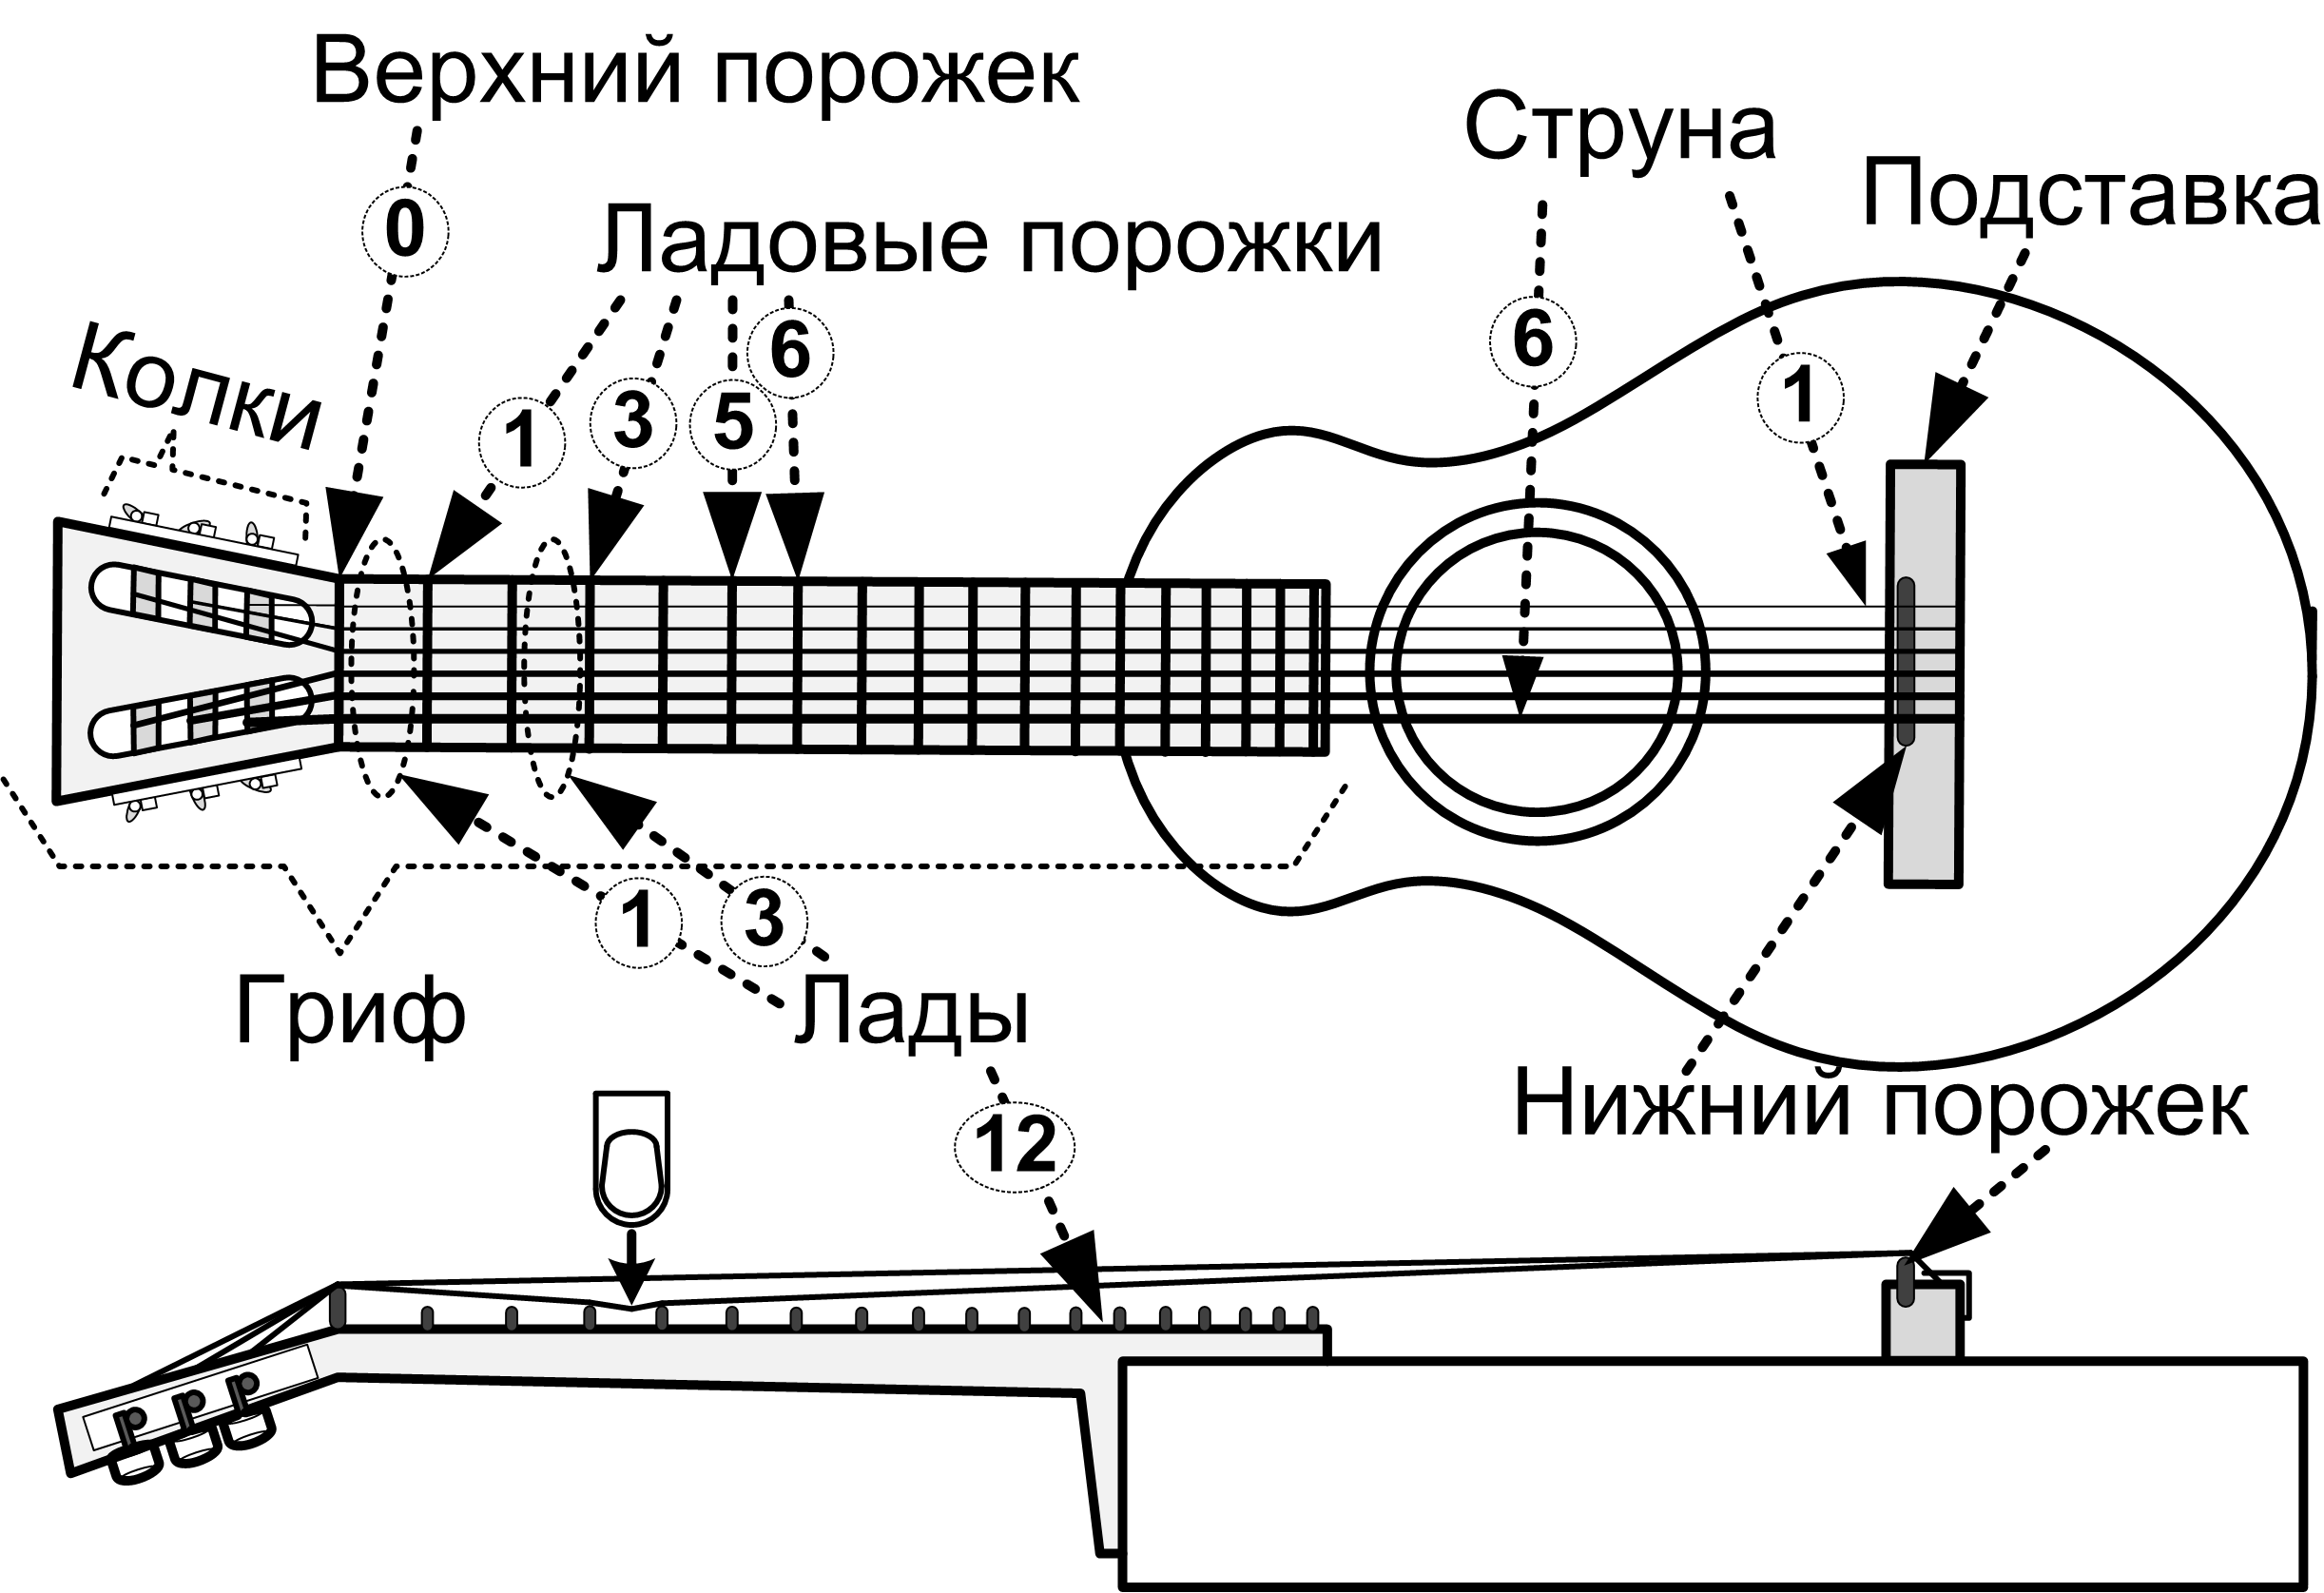
\includegraphics{fig/guitar-play} 
    \caption{Струны на гитаре}\label{fig:music:tone:guitar-play}
\end{figure} 

Гитара\index{гитара}, названия основных частей которой отражены на рисунке \ref{fig:music:tone:guitar-play}, использует оба способа управления высотой звука. Струна одним концом крепится к подставке, а другим наматывается на колок --- специальный механизм, позволяющий очень плавно регулировать натяжение струны. При этом звучащая часть струны одним концом опирается на верхний порожек, а вторым --- на нижний порожек на подставке. Чтобы укоротить звучащую часть струны, практически не меняя её натяжения, достаточно прижать её пальцем к металлическому ладовому порожку на грифе. Это называется <<зажать струну на ладу>>, например, на рисунке \ref{fig:music:tone:guitar-play} струна <<зажата на четвёртом ладу>>.

Перед тем как играть, гитару настраивают, то есть регулируют нужным образом натяжение струн, которое во время игры уже не меняется. Гитарист извлекает звуки разной высоты, прижимая струну к металлическим ладовым порожкам на грифе, тем самым укорачивая её: быстро и просто. Об устройстве и настройке гитары мы поговорим подробнее в разделе \ref{ch:guitar}.

Важно понять, что струна порождает не одну звуковую волну определенной частоты, а сразу бесконечное их множество, потому что независимо друг от друга колеблются\index{струна!колебания} половинки струны, её трети, четверти и так далее!

\begin{figure}[!ht]
    \centering
    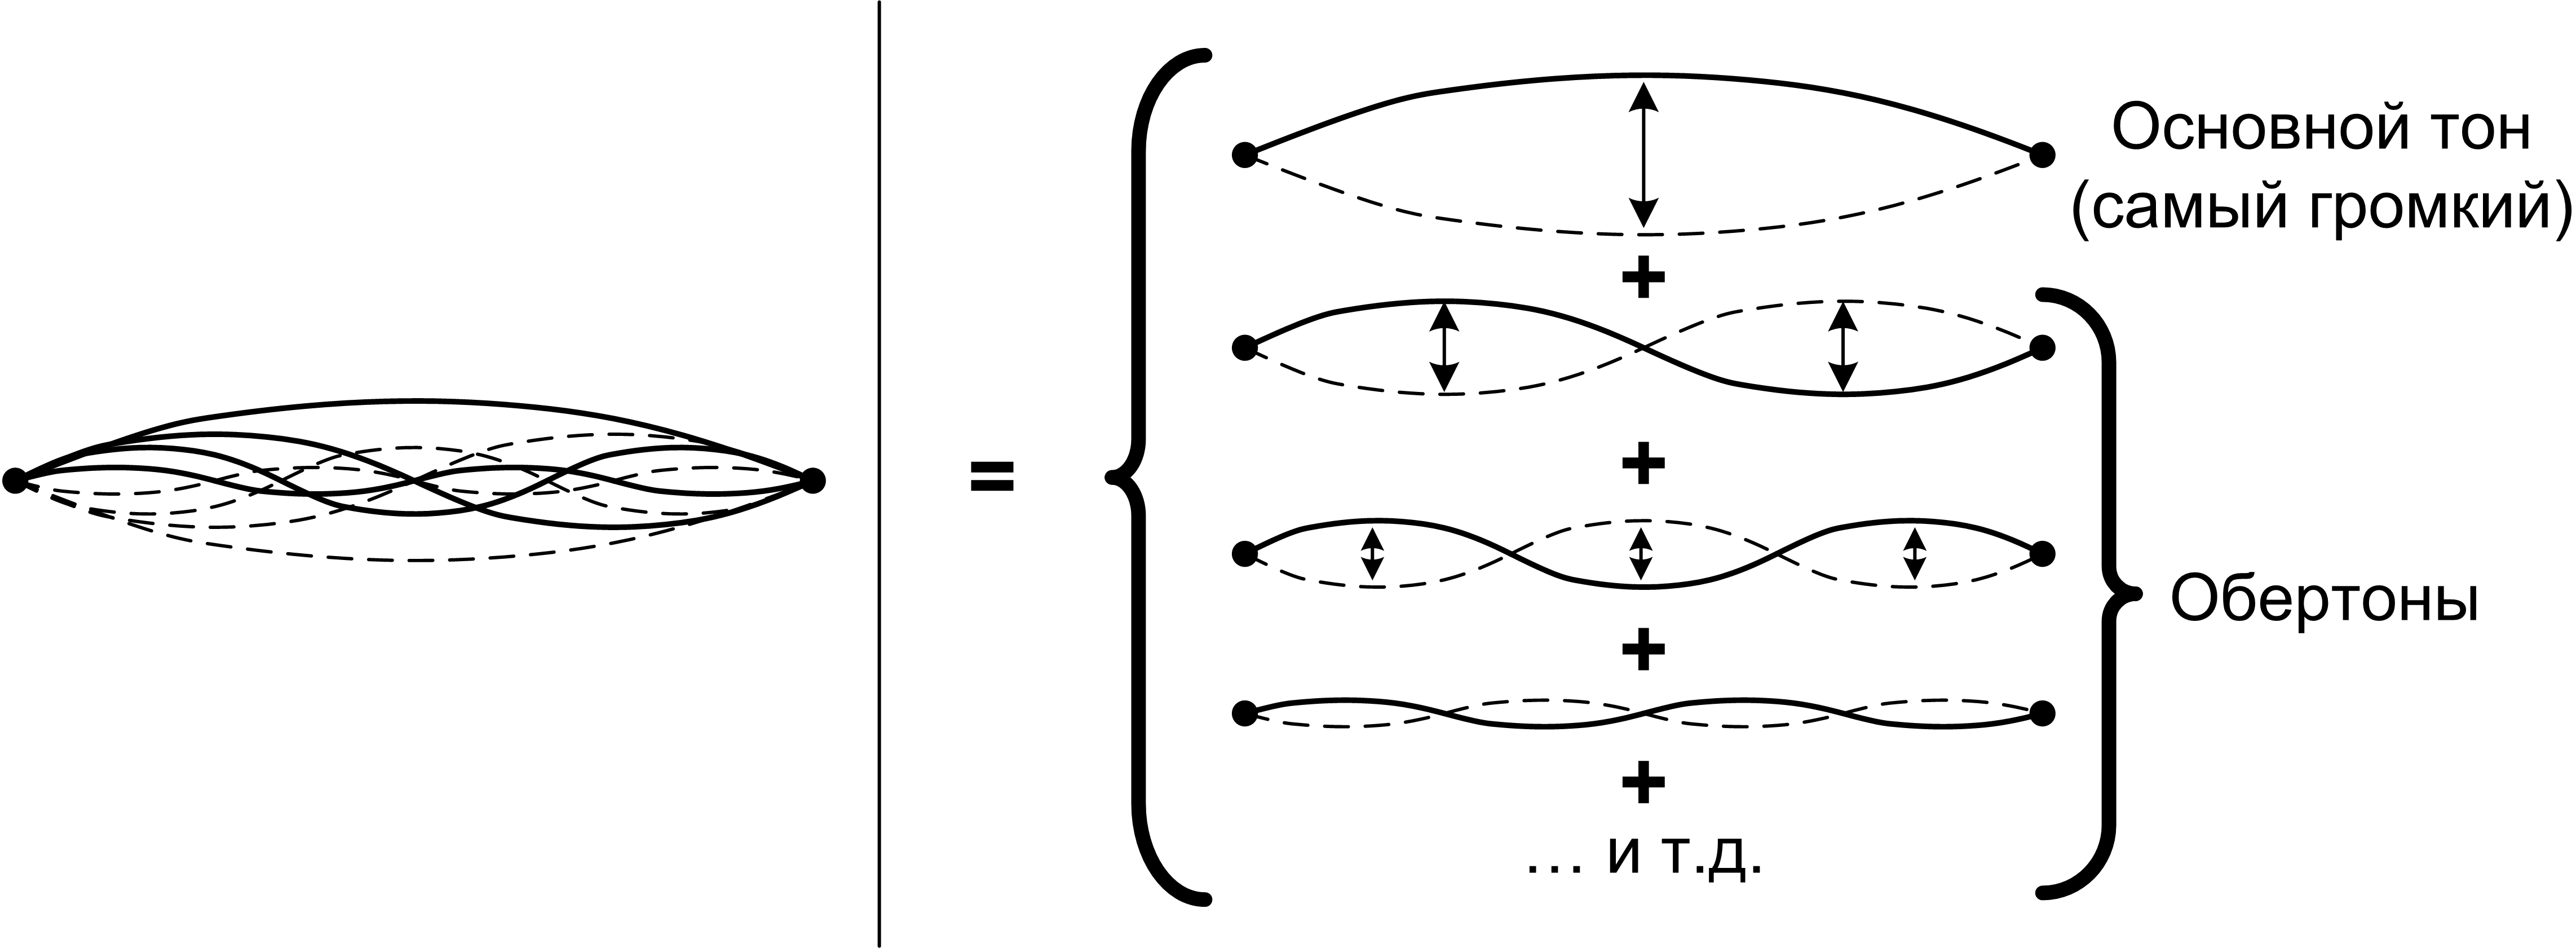
\includegraphics[width=\textwidth]{fig/string-moving} 
    \caption{Колебания струны}\label{fig:music:tone:stringmoving}
\end{figure} 

На рисунке \ref{fig:music:tone:stringmoving} колебания струны разложены на составляющие (справа от знака равенства). Максимальную амплитуду колебаний имеет так называемый \emph{основной тон}\index{тон основной!звука}, когда струна колеблется по всей длине. Основной тон слышен громче всех. Остальные составляющие принято называть \emph{обертонами}\index{обертон}. Они звучат тише основного тона, но придают звуку особую окраску. Каждая гитара имеет свой особенный <<голос>> именно благодаря обертонам.

\begin{Example}[Эксперимент: обертоновая окраска звука]
    Мы уже знаем, что изданный струной звук --- это <<смесь>> из <<чистых>> колебаний разных частот. А вот в каких пропорциях будут <<смешаны>> обертоновые ингридиенты зависит во многом от того, в каком месте щипнуть струну.
    
    Для эксперимента нам потребуется гитара. Будем играть на шестой, самой низкой басовой струне и постараемся все звуки извлекать одинаково энергично. Легко положите пальцы левой руки на струны с 1-й по 5-ю, таким образом заглушив их. Для извлечения звука лучше использовать медиатор, кончик ногтя или любую другую подходящую пластинку --- так звончее. Сравните свои слуховые ощущения от щипка струны в разных местах (см. рисунок \ref{fig:music:tone:obertone-color}). Кроме того, колебания шестой струны хорошо заметны визуально (она как бы <<размазывается>> в воздухе). Так что советую не только прислушаться, но и присмотреться.
    \begin{itemize}
        \item Щипнув струну ровно посередине (точно над 12 ладовым порожком) вы услышите звук, напоминающий звук варгана. Визуально, размах колебаний струны над двенадцатым ладом максимален.
        \item Сыграв в обычном месте, над ближним к нижнему порожку краю розетки, вы услышите более <<мягкий>>, бархатистый звук. Размах колебаний заметно уменьшился.
        \item От щипка в двух-трех сантиметрах от нижнего порожка звук получается резким и звенящим. Колебания струны в середине стали еще меньше.
    \end{itemize}
    
    В первом случае мы защипнули струну в самой <<амплитудной>> (размашистой) точке основного тона и практически вся энергия ушла в основной тон, а обертонам ничего не досталось. Сместив щипок ко краю розетки, мы добавили энергии низкочастотным обертонам. А щипнув струну возле нижнего порожка энергия ушла в обертоны высокой частоты. См. рисунок \ref{fig:music:tone:obertone-color}.
    
    \begin{figure}[!ht]
        \centering
        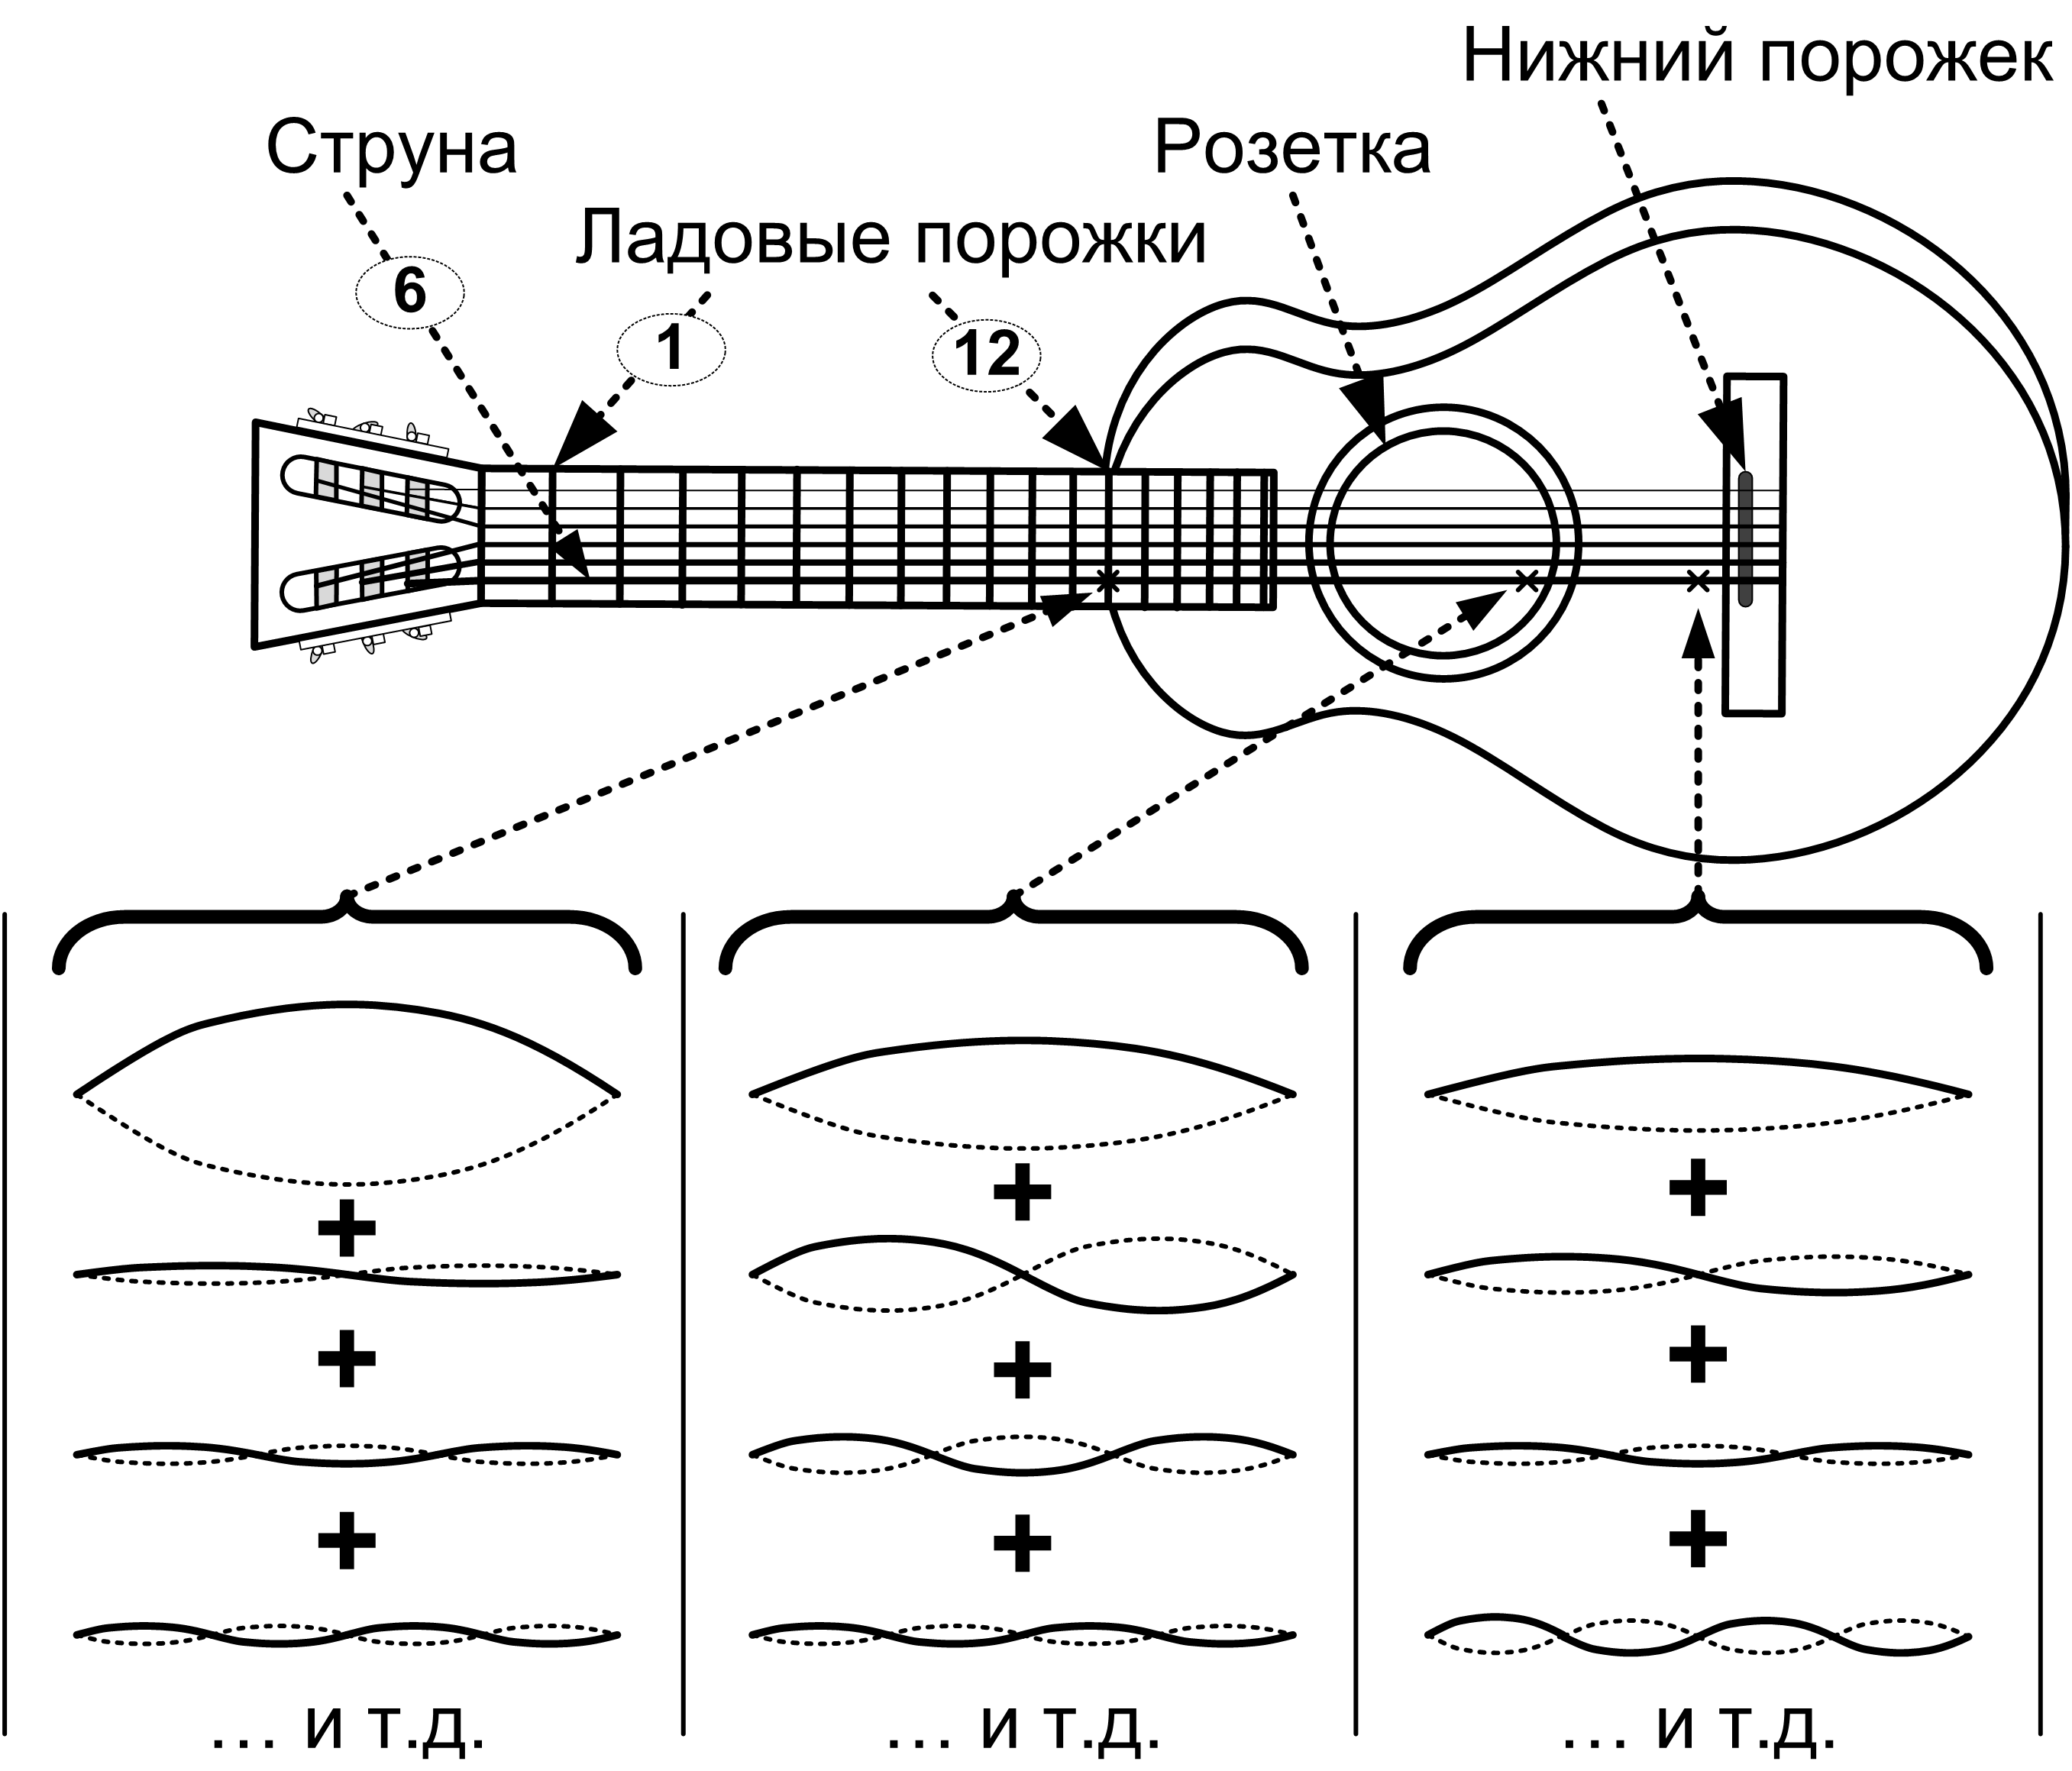
\includegraphics{fig/obertone-color} 
        \caption{Тембровая окраска звука в зависимости от места щипка}\label{fig:music:tone:obertone-color}
    \end{figure} 
\end{Example}


\begin{Definition}[Частота колебаний струны]
    Если при неизменном натяжении в $N$ раз \emph{укоротить} звучащую часть струны, то частота издаваемого основного тона \emph{увеличится} в $N$ раз.
\end{Definition}

Когда говорят о высоте звука струны, то по умолчанию имеют в виду именно частоту колебаний \emph{основного тона}.

Чтобы создавать музыку, используют ограниченный набор так называемых \emph{музыкальных} звуков\index{звук!музыкальный}, отличающихся по высоте. При этом высота (частота) музыкальных звуков должна укладываться в строгую математическую систему --- \emph{музыкальный строй}\index{строй}. Таких систем (строёв) сложилось несколько\footnote{Например, Чистый строй, Пифагоров строй}, но мы ограничимся только тем строем, который положен в основу конструкции гитары. Он называется <<равномерно темперированным>>.

Но прежде чем начать разбираться с равномерно темперированным строем, нужно определить очень важное понятие: \emph{расстояние} между двумя звуками. То есть ввести меру отличия одного звука от другого по \emph{высоте} (по частоте колебаний основного тона). 

Если укоротить струну вдвое, то частота её колебаний вдвое увеличится. Сыграйте звук сначала на открытой\index{струна!открытая} (то есть не зажатой ни на каком ладу) струне, потом на её половинке\footnote{На гитаре это можно сделать, зажав струну на 12-м ладу}, и вы услышите два совершенно различных звука. Но если сыграть эти звуки одновременно, то почти сольются: <<на слух>> один звук просто потеряется в другом. Это объяснимо: глядя на рисунок \ref{fig:music:tone:stringmoving} можно убедиться в том, что звук, издаваемый половинкой струны, полностью <<содержится>> в обертонах открытой струны. Самый громкий обертон в составе звука имеет частоту вдвое меньшую, чем основной тон.

\begin{Definition}[Октава]
    Два звука находятся друг от друга на расстоянии \emph{октавы}\index{октава}, если их частоты отличаются в \emph{два} раза. Звук \emph{выше на октаву}, если его частота \emph{в два раза больше} частоты исходного звука. 
\end{Definition}

Почему эта мера расстояния названа <<октавой>> мы разберемся в разделе \ref{ch:harmony:interval}, а сейчас отметим, что октава --- очень большое расстояние, тогда как человеческое ухо воспринимает куда меньшие изменения частоты. В равномерно темперированном строе октава делится на 12 частей, а каждая отдельная частичка октавы уже неделима и называется <<полутоном>>\index{полутон}.

\begin{Example}[Октава на грифе гитары]
    Давайте немного разбавим теорию практикой: возьмите гитару и линейку (можно даже просто суровую нитку). Измерьте длину любой струны от верхнего порожка до нижнего (см. рисунок \ref{fig:music:tone:guitar-play}, если возникли трудности). Поделите длину струны на два (сложите нитку вдвое) и убедитесь, что середина струны находится над 12-м ладовым порожком. Звук, извлеченный на 12-м ладу, на \emph{октаву выше} звука открытой струны. Звук, извлеченный на 1-м ладу, \emph{выше} звука открытой струны на \emph{полутон}.
\end{Example}

Заметим, что мы имеем дело с геометрической прогрессией: частота звука на октаву выше исходного \emph{в два раза} больше частоты исходного звука\footnote{Физики, привет, слыхали о децибелах?}. Если мы зафиксируем некоторую частоту $f_0$ <<базового>> звука, то частота звука на одну октаву выше будет $f_0\cdot 2$, а в общем случае, частота звука $f_m$, который на $m$ октав выше <<базового>>:
\[
    f_m = f_0\cdot 2^m.
\]

Чтобы поделить октаву на $12$ частей, нужно выбрать такое основание геометрической прогрессии $b$, чтобы $b^{12} = 2$, а значит:
\[
    b = \sqrt[12]{2} \approx 1,059463.
\]

Итак, подходим к сути. 
\begin{Definition}[Музыкальный строй]
    \emph{Музыкальный строй}\index{строй!музыкальный} --- это правила отбора частоты колебаний основного тона для звуков, которые будут называться \emph{музыкальными}. 
\end{Definition}    

Только такие, и никакие другие, звуки можно извлекать из правильно \emph{настроенного} музыкального инструмента\index{инструмент музыкальный}.

Из всего диапазона частот звуков, слышимых человеком, нужно отобрать конечное множество правильных, <<музыкальных>>. В равномерно темперированном строе\index{строй!музыкальный!равномерно темперированный} это делается так:
\begin{itemize}
    \item Фиксируется частота эталонного\footnote{Это на самом деле международный стандарт. ISO 16. ISO --- International Organization for Standardization, международная огранизация по стандартизации. Эталонные 440 Гц называют также Штудгардской высотой (Stuttgart pitch)\index{Штудгардская высота}, иногда обозначают A440 или A4} \emph{музыкального} звука: 440 Гц. Гитарная струна издавая этот звук, будет совершать 440 полных колебаний в секунду\footnote{Вполне допускается вольность принять за Ля первой октавы любую частоту из интервала от 430 до 450 герц. Многие фанатики утверждают, что Ля в 432 Гц одобрена Богом (и оздоравливающе действует на организм), а утвержденная стандартом 440 Гц --- от Сатаны (и разрушает психику)}. Эталонную частоту обозначим: 
    \[  
        f_{A4}=440\text{Гц}.
    \]
    
    Пояснию, что такое $A4$\index{A4} --- это латинское обозначение для ноты ЛЯ (которая по-латински обозначается --- $A$) четвертой по счету октавы. \emph{Нота} --- это способ обозначения \emph{музыкального} звука. О нотной грамоте поговорим в разделе \ref{ch:notes:names}.
    
    \item Вводится правило получения частоты $n$-го музыкального звука на основе эталонной частоты. Частота $n$-го музыкального звука $f_n$ будет определяться так: 
    \begin{equation}
        f_n = f_{A4}\cdot({\sqrt[12]{2}})^n, \label{eq:music:tone:frequency}
    \end{equation}
    где целое число $n$ может принимать и отрицательные значения, чтобы получить музыкальные частоты меньше 440 Гц.
\end{itemize}

В равномерно темперированном строе частота от звука к звуку повышается в \emph{геометрической} прогрессии. То есть частота звука, который на \emph{полутон} выше исходного ($n$-го), в 
\[
    \frac{f_{n+1}}{f_n} = \frac{f_{A4}\cdot(\sqrt[12]{2})^{(n+1)}}{f_{A4}\cdot(\sqrt[12]{2})^n} = \sqrt[12]{2}
\] 
раз больше частоты исходного звука. Кстати, в такой же пропорции находятся и расстояния между соседними ладовыми порожками гитары\footnote{Подробнее см устройство гитары в разделе \ref{ch:guitar}}.

А если музыкальный звук на 12 полутонов (т.е. на октаву) выше исходного, то его частота будет в два раза больше частоты исходного звука:
\[
    \frac{f_{n+12}}{f_n} = \frac{f_{A4}\cdot(\sqrt[12]{2})^{(n+12)}}{f_{A4}\cdot(\sqrt[12]{2})^n} = (\sqrt[12]{2})^{12} = 2.
\]

\begin{figure}[!ht]
    \centering
    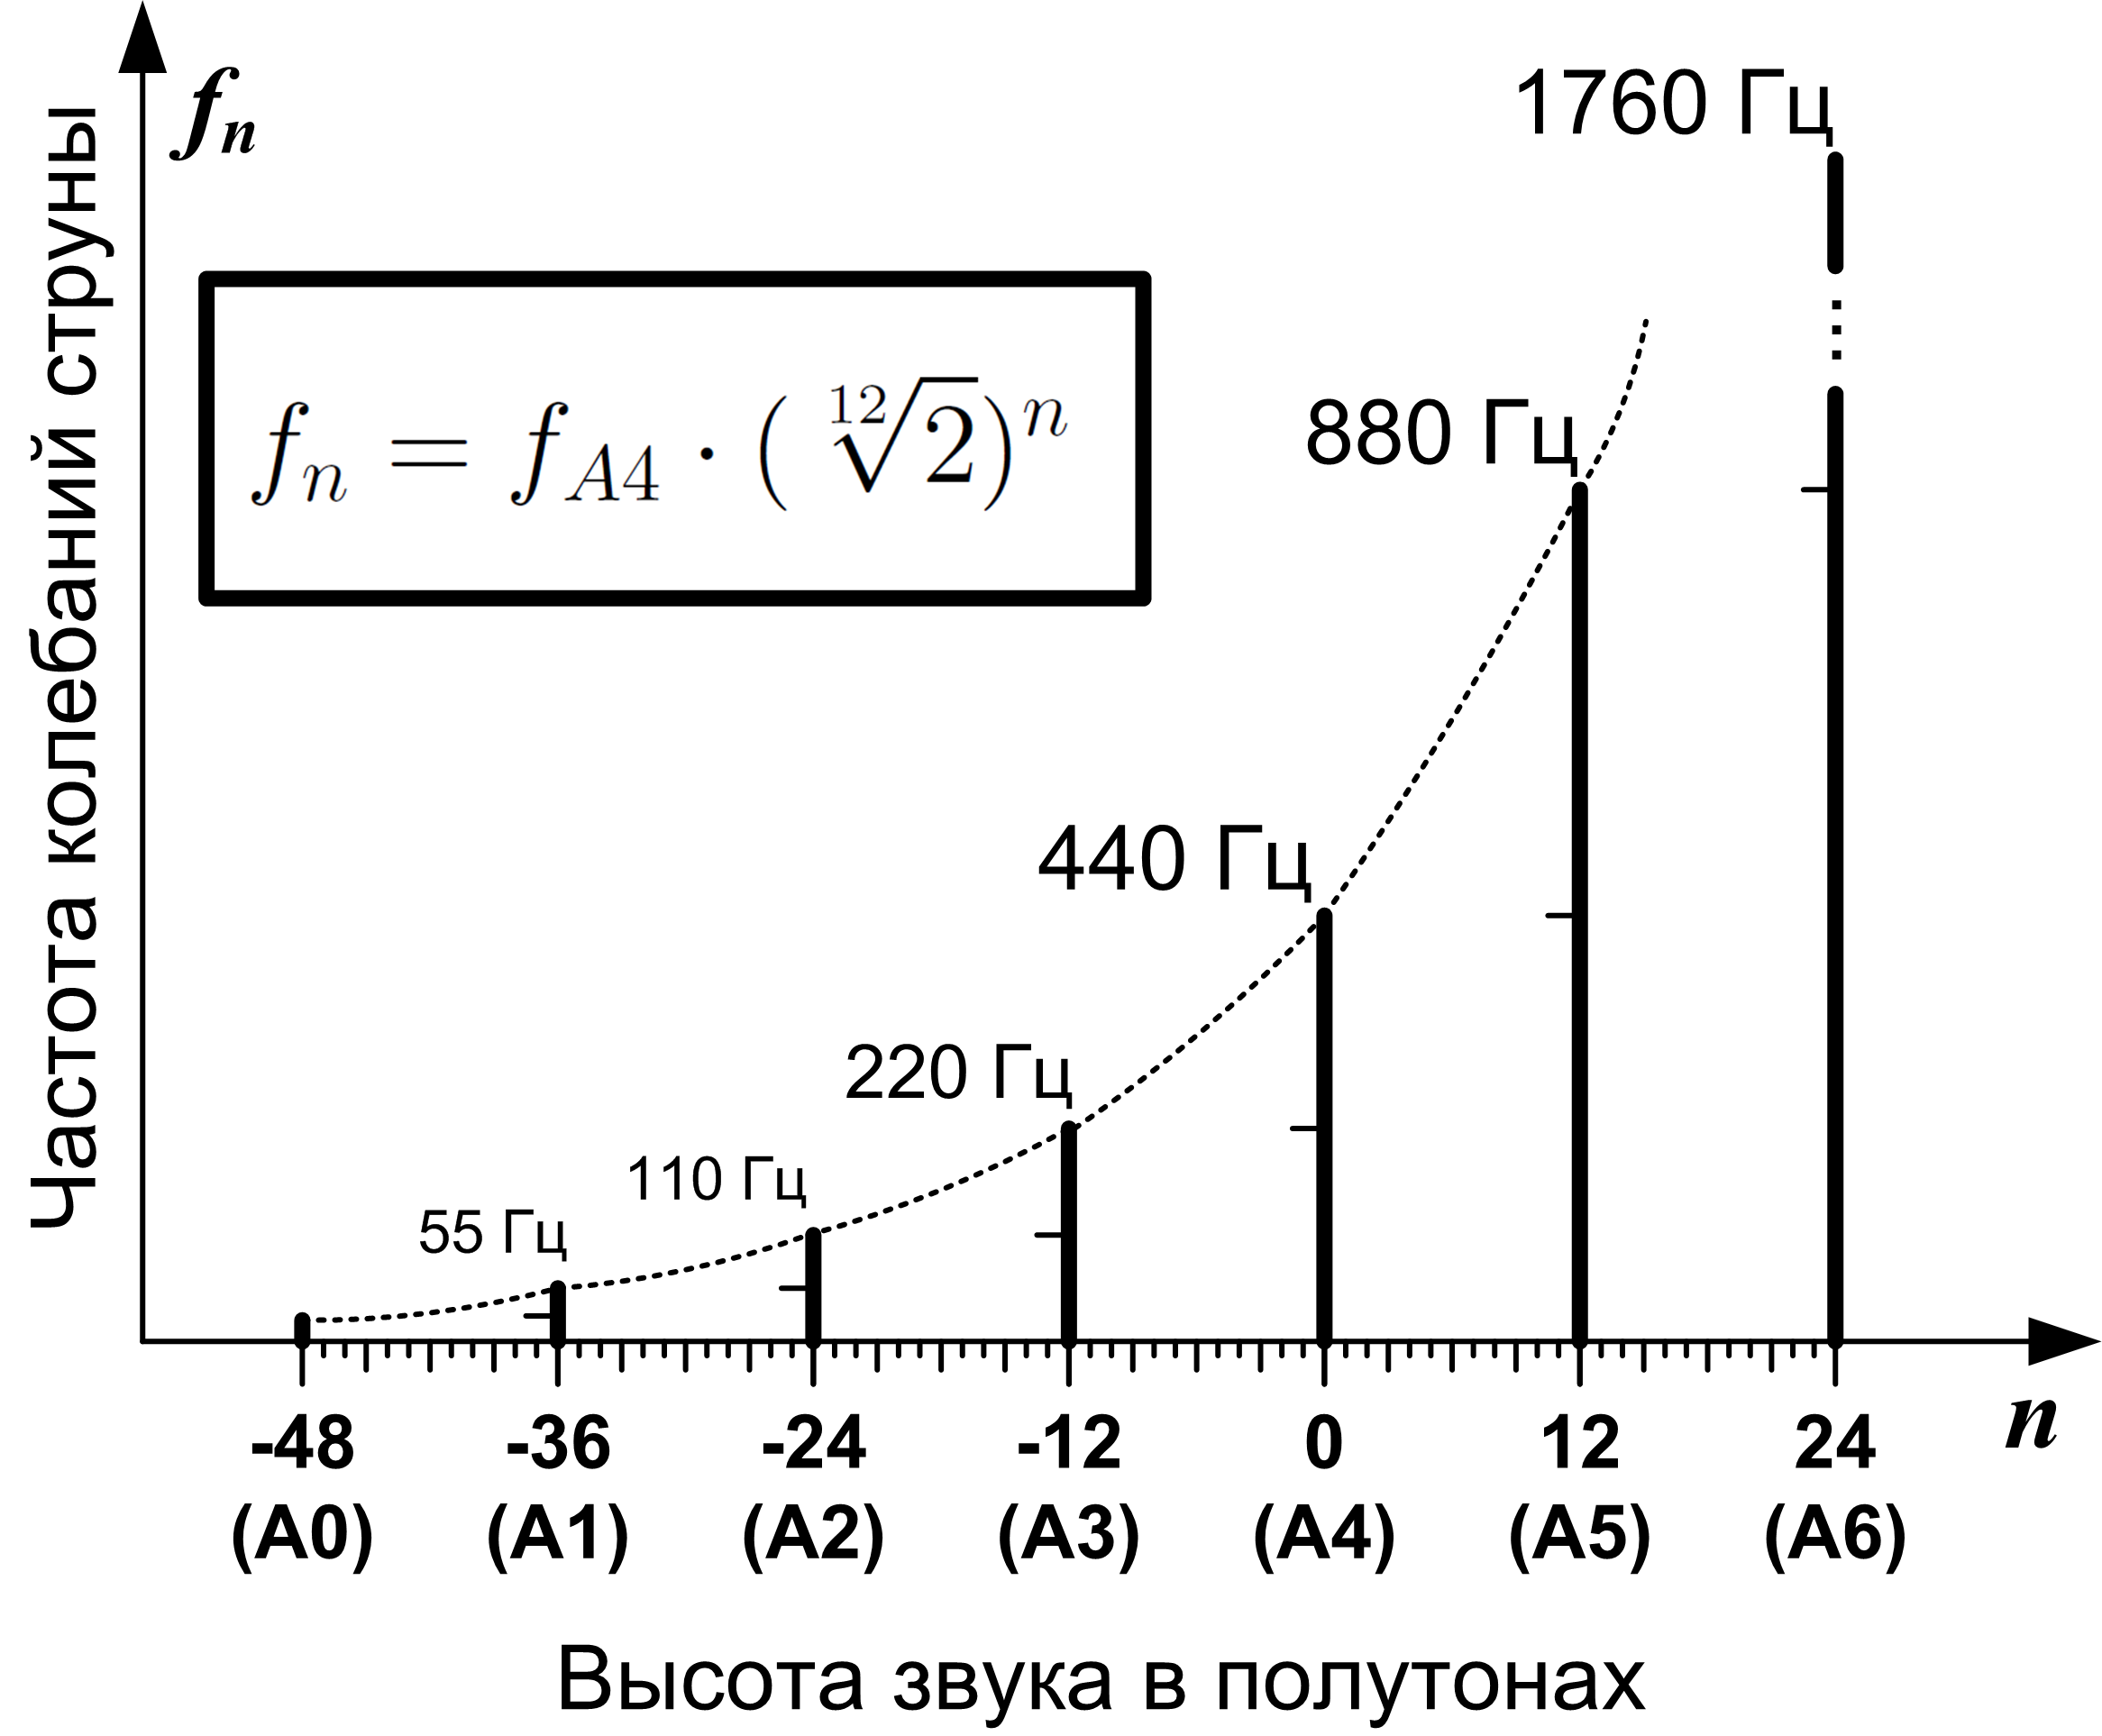
\includegraphics{fig/tempered} 
    \caption{Равномерно темперированный строй}\label{fig:music:tone:tempered}
\end{figure} 

Вот такие строгие правила отбора нужных звуков по частоте сложились в современной музыке. 

\begin{Example}[Сколько всего музыкальных звуков?]
    Полезно будет грубо прикинуть общее количество \emph{музыкальных} звуков\index{звук!музыкальный!количество}, доступных человеку для восприятия. Напомню, что нижний предел восприятия примерно 16 Гц, а верхний --- 20000 Гц. 
    
    Возьмем звук 16 Гц за основу (начало) <<нулевой>> октавы и прикинем, сколько всего будет октав, покрывающих слышимый человеком диапазон. Начало следующей (первой) октавы будет $16\cdot 2 = 32$ Гц, а в общем случае, $m$-я октава будет начинаться со звука частотой $16\cdot 2^m$ Гц. Даже простым перебором $m$ легко установить, что начало 11-й октавы находится уже за пределами восприятия: 
    \[
        (16\cdot 2^{11} = 16\cdot 2048 = 32768) \ge 20000.
    \]
    
    Т.е. всего имеют смысл примерно 11 октав, в каждой по 12 звуков, так что всего музыкальных звуков примерно 132, да и то не все <<нормальные люди>> смогут их услышать.
\end{Example}

На графике (см. рисунок \ref{fig:music:tone:tempered}) показана зависимость частоты основного тона для $n$-го звука. Музыканты работают только с горизонтальной осью --- простой упорядоченной последовательностью музыкальных звуков и совсем не задумываются о частотах. Кроме того, вместо целых чисел (номеров музыкальных звуков) у них сложилась особая система обозначений --- \emph{нотная грамота}. Например, вместо $0$-й звук (на рисунке \ref{fig:music:tone:tempered}) музыкант скажет: нота ЛЯ первой октавы, вместо $2$-й --- нота СИ первой октавы,\ldots, $12$-й --- снова ЛЯ, но второй октавы. И т.д. Словом, учиться понимать музыкантов будем в разделе \ref{ch:notes:names}.


\section{Маршируем или вальсируем? Правильная громкость}
\label{ch:music:volume}

<<Аты-баты, шли солдаты, аты-баты на базар!>> Марш\index{марш}. Длительный пеший переход уныл без музыки. Ритм чеканим ногами: 
\begin{center}
    Левой--Левой--Раз-два-Три--,\ldots 
\end{center}
Знакомо? А что касается музыки, чтобы веселее шагалось, при наличии оркестра, лучше прям барабаном вжахнуть под левую ногу. Это называется \emph{акцентом}\index{акцент}. 

<<Крутится, вертится шар голубой, Крутится, вертится над головой, Крутится, вертится, хочет упасть, Кавалер барышню хочет украсть>>. Вальс\index{вальс}. 
\begin{center}
    Раз-два-три, Раз-два-три,\ldots 
\end{center}
В случае вальса какой-нибудь контрабас громко мурявкает на <<Раз>>.

Периодичность --- это часть нашей жизни. Пульсирует в жилах кровь, тикают секунды в часах, рассветы сменяются закатами, лето --- зимой. Вот и музыка пульсирует, живёт акцентами. Живёт по своему, где-то громче, где-то тише, и конечно живёт не только вальсами и маршами.

Одним словом --- ритм\index{ритм}! Ритм нужно акцентировать. Лучше барабаном, наверное, одним из самых древних после голоса музыкальных инструментов. Но раз уж мы выбрали гитару\ldots

Самый дешевый и сердитый способ сделать акцент на звуке --- выделить его громкостью. Обычный способ для гитары сделать акцент --- не просто сильнее дернуть струну, а сыграть басом\index{бас}, то есть низким звуком. Басовые струны --- тяжёлые, а значит они звучат не только ниже (т.е. медленней колеблются), но и громче (колеблются с б\'{о}льшей амплитудой).

Конечно, громкость --- не единственный способ сделать акцент. Звук может обратить на себя внимание, например, необычными обертонами (музыканты называют это \emph{тембровой} окраской звука). Сыграйте флажолет (см. раздел \ref{ch:tricks:flageolet}) и оцените \emph{необычность} его звучания.


\section{Еще и глушить надо? Правильное время}
\label{ch:music:rythm}

Звуки сменяют друг друга, и музыка течёт во времени. 

Гитара позволяет извлекать несколько звуков сразу. Два звука, извлеченных одновременно\footnote{Ну, или очень быстро друг за другом. Например, при игре <<боем>> (<<чёсом>>) --- правая рука просто бъет вверх-вниз по всем струнам с определенным ритмом, а левая только успевает зажимать струны. При этом на каждый бой звучит аккорд, но струны, строго говоря, начинают звучать не одновременно}, называют \emph{интервалом}\index{интервал}. Три и более --- \emph{аккордом}\index{аккорд}.

Интересно, что результат смешения звуков разной высоты, может быть как приянтым, так и неприятным на слух. Неприятное смешение звуков называется \emph{диссонансом}\index{диссонанс}. Замечательно то, что заранее и абсолютно точно можно сказать как тот или иной интервал или аккорд повлияет на слушателя. Собственно музыка --- это искусство игры на нервах: создавая периоды приятных и неприятных звуковых ощущений, композитор добивается определенного настроения слушателя. Подробнее о теоретических основах гармонии мы поговорим позже, в главе \ref{ch:harmony}.

Колебания гитарной струны быстро затухают, то есть звук быстро теряет громкость. И чаще всего не нужно думать о том, как вовремя заглушить струну: к тому моменту, когда вы извлечёте из гитары следующий звук, предыдущий затихнет сам. Но в музыкальном мире всё относительно --- например, басовые струны звучат громче и дольше остальных, а стало быть их звук будет накладываться на звуки, извлечённые позже. Если это будет портить музыку, то в нотах композитор поставит специальные пометки, указывающие на необходиомсть специально глушить соответствующие звуки. На гитаре заглушить струну несложно: достаточно легко прикоснуться к ней пальцем.

Так как музыка пульсирует, укладывается в определенный ритм, создаваемый акцентами, то звуки действительно должны появиться и угаснуть в определённое время, чтобы поддержать эту пульсацию. В музыке введено понятие \emph{такта}\index{такт} --- фиксированного периода времени, через который обязательно появляются самые сильные акценты. И длительность отдельных звуков в музыке измеряется долями такта, то есть звук может прозвучать: половину такта, четверть, восьмую долю, шестнадцатую и тд. Чаще всего такт делят степенями двойки, но нередко бывает, что звук длится треть такта, пятую или седьмую его часть.

Ещё раз отмечу, что, теоретически, струна, если её не заглушить специально, \emph{звучит}, затухая, вечно. С практической же точки зрения \emph{музыкальный} звук обычно \emph{длится} до тех пор, пока не прозвучит куда более громкий следующий звук. Например, если нужно сыграть звук, длящийся четверь такта, то музыканту (если нет особых пометок) вообще не нужно глушить струну, а достаточно просто вовремя извлечь \emph{следующий} звук.


\section{А радость где? Правильное отношение к правилам}
\label{ch:music:rules}

Правила существуют для того, чтобы их нарушать. Радость она ведь от озорства. Так что нарушать нужно искромётно и тонко, с хитрецой. Так, чтобы вроде и нарушил, да ловко так, что и простить можно! Не закон Божий, в конце-то концов\ldots

Существует много озорных заигрыванй с правилами. Ну, например, приёмчик <<подтяжка>> струны\index{подтяжка струны}: струна пальцем левой\footnote{Речь о правшах. Левши, вы знаете, что делать!} руки зажимается на ладу и играется как обычно, но, пока она звучит, палец, не ослабляя нажим, сдвигает (в пределах 1-2 см) струну вверх или вниз по порожку лада. Можно даже поелозить вверх-вниз. От таких действий натяжение струны меняется и звук плавно повышается, обычно в пределах долей полутона --- это уж как силушка богатырская позволяет.

И таких хулиганств на гитаре придумано немало: всякие там вибратто, легато (hammer-on, pull-off), тэппинг и т.д. Забавно, что и вокруг хулиганств постепенно формируются свои правила: мол вот так <<подтяжку>> правильно играть, а так --- нет\ldots Ага, ага, не вопрос!

Заигрывают с ритмом, например, когда гитаристу вдруг захочется барабанов, он может побарабанить по гитаре\footnote{Барабанить по гитаре --- в каком-то смысле уже классика. На гитару даже наклеивается специальная накладка в районе розетки, по которой уже давно подстукивают пальцами горячие испанцы --- гольпеадор. Посмотрите видео про румбу на канале Игоря Горохова \cite{url:gorohovIgor}} --- фингерстайл\ldots Заигрывают и с длительностью звука, например, если электрогитару приблизить к усилителю звука, то усиленный звук струны, естественно звучаший в резонанс со струной, будет ещё сильнее <<расшатывать>> струну, звук которой в свою очередь будет усилен. Обратная связь\index{обратная связь}. Струна будет звучать вечно, только ток на усилитель подавай!

Эх, прям на философию потянуло. Может потому-то и движется жизнь вперед? На месте хулиганств рождаются новые правила, порождающие очередные хулиганства. Обратная связь, ага. В общем без правил похулиганить не получится, а стало быть и радости никакой.

Напоследок: нарушать правила следует тогда, когда и знания, и мастерство позволяют это делать \emph{элегантно}.